\documentclass{IEEEtran}
\usepackage[latin1]{inputenc}
\usepackage{amsmath}
\usepackage{amsfonts}
\usepackage{amssymb}
\usepackage{graphicx}
\usepackage{subfig}
\usepackage{floatrow}

\author{
	\IEEEauthorblockN{MatthewBrown\\}
	\IEEEauthorblockA{Machine Learning Final Project\\University of Idaho}	
}
\title{Neural Net Accuracy Degradation from Noisy Input}
\begin{document}
	\maketitle
	\begin{abstract}
		This paper outlines an experiment preformed as a final project for the machine learning class at the University of Idaho. For this experiment the question was asked ``can a hopfield neural network combination filter out noise better than a neural network alone?" The MNIST handwritten digit dataset was used for this experiment due to its ease of access and its size.
		
		Results of the experiment found that a hopfield neural network combination is resilient through more than 25\% noise that is injected into the data, where a neural net alone begins loosing accuracy immediately.
	\end{abstract}
	
	\section{Introduction}
		Throughout the machine learning course students learned a number of different techniques for classifying data. Two mechanisms that stood out to me were the neural network and the hopfield network. A neural network is a mechanism for classifying data based on a system of mathematical weights that determine the classification of a data set by determining which data points are most significant. A hopfield network is a recurrent neural network that can be trained to ``remember" various data points and can be used to recall the data points at a later time. Hopfield networks are especially good at receiving a noisy image and recalling a clean image that matches the noisy image best.
		
		For this experiment the MNIST handwritten digit data set was used. Images from the data set were made noisy and fed through the hopfield network then through the neural net in an attempt to identify the digits through the noise. The overall research question to this project was ``can a hopfield neural network combination filter out noise better than a neural network alone?"
		
	\section{The Experiment}
		The experiment preformed for this paper is composed of two parts. For first part, a neural net's accuracy was tested while slowly increasing the amount of noise in the input data. In the second part of the experiment noisy data was first fed through a hopfield network then through the neural net. For bot experiments both single-layer and multi-layer neural nets were used. In this section the details of the components used will be explained as well as the results for the experiment.
		\subsection{The Data}
			The data used for this experiment is the famous MNIST handwritten digit dataset \cite{MNIST}. This data set was selected for its size and the amount of research that already exists on it. This dataset contains around 70,000 handwritten digit samples ranging from 0-9. The data was split into a training set of 60,000 images and a testing set of 10,000 images. All samples are 28 X 28 pixel pictures. 
			
			For this experiment each pictures was broken down into its 784 greyscale pixels, ranging from 0 to 1, and were converted into black and white. Once the data was converted to the desired format, a random noise algorithm was applied to the data in order to create a ``fuzzy" version of the image. Because the pixels for this experiment are in black an white simple bit flips are preformed to create the noise. Figure \ref{cleanSeven} and \ref{dirtySeven} illustrate the effect of the noise function applied to the data. 
			
			For the first part of the experiment data is fed into the neural nets directly. In the second part the data is first fed through a hopfield network. The resulting or recalled data is then fed through the neural net.
			
			\begin{figure}
				\begin{floatrow}
					\ffigbox{
\includegraphics[scale = 0.8]{clean.png}}{\caption{Clean Data}\label{cleanSeven}}
					\ffigbox{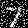
\includegraphics[scale = 0.8]{dirty.png}}{\caption{Noisy Data}\label{dirtySeven}}
				\end{floatrow}
			\end{figure}
			
		\subsection{The Neural Nets}
			As previously stated two different types of neural nets were used in this experiment. Tensor Flow was used for modeling the neural nets. Both neural nets were trained with the clean versions of the training data-set provided by MNIST.
			
			The first neural net used was a single layer neural net. This neural net uses a weight matrix of 784 rows by 10 columns. The number of rows is determined by the size of the input vector while the number of columns is determined by the size of the output vector, so 784 pixel pictures are turned into a 10 point vector where the position of the identified value is one and all other bits are off. A softmax regression model is used for training and the accuracy of the neural net is calculated by averaging the results \cite{Tensor1}.
			
			The multi-layer neural net is a bit more complicated. The multi-layer neural net uses 2 convolutional layers, a densely connected layer and a readout layer to analyze the data. The convolutional layers split the data into 5 X 5 sections for the first layer and into 7 X 7 sections in the second layer. This allows the neural net to analyze the picture in sections. The next layer is the densely connected layer which combines the second layer into 1024 connected neurons, allowing analysis of the picture as a whole. The final layer, the readout layer, converts the data into the 10 bit vectors that indicate the final decision of the neural net \cite{Tensor2}. 
		
		\subsection{The Hopfield Network}
			The hopfield network used in the second part of the experiment is a simple hopfield network with a 784 x 784 weight matrix. The weight matrix was trained by using the ``average" of each type of picture. The averages were calculated by pixel-wise adding each image for each given type and performing a scalar divide on the resulting matrix. It is important to note that for the second part of the experiment only pictures of 0's and 1's were used due to a limitation of the hopfield network.
			
		\subsection{Extra preliminary information}
			Both parts of the experiment were run on a virtual machine with 20 CPU cores and about 16Gb of RAM. Multiprocessing was used to speed many of the independent calculations, such as applying noise to the data samples. Part 1 took approximately 20 minutes to run while part 2 took a little over an hour. Python is used for all experiments as well.
			
		\subsection{Part 1}
			For the first part of the experiment all 10 digits were fed through both the single and multi-layer neural nets. Using clean data the single layer neural net averaged about 90\% accuracy while the multi-layer neural net averaged about 96\% accuracy. Once a base line was established, noisy data was run through the neural net to observe a loss of accuracy. The noisy data started with small amounts of noise being applied and was steadily increase over the course of the experiment.
			
			For the single layer neural net accuracy loss was apparent almost immediately. An apparent rate of 
			\begin{equation*}
			y = -0.0003x4 + 0.0241x3 - 0.5927x2 + 1.6172x + 90.164
			\end{equation*}
			formed where y is the expected accuracy and x is the percent change of the noise data when compared to its original. The multi-layer neural net also appeared to have accuracy loss right away; however, it appears that the overall rate of accuracy loss was slower than its single layer counterpart. The rate of accuracy loss appears to be around
			\begin{equation*}
			y = 0.0002x^4 - 0.0078x^3 - 0.0141x^2 - 0.5348x + 96.124
			\end{equation*}
			which seems to have a slower rate of decay. Figure \ref{part1} illustrates the accuracy decay of both neural nets.
			
			\begin{figure}
				\centering
				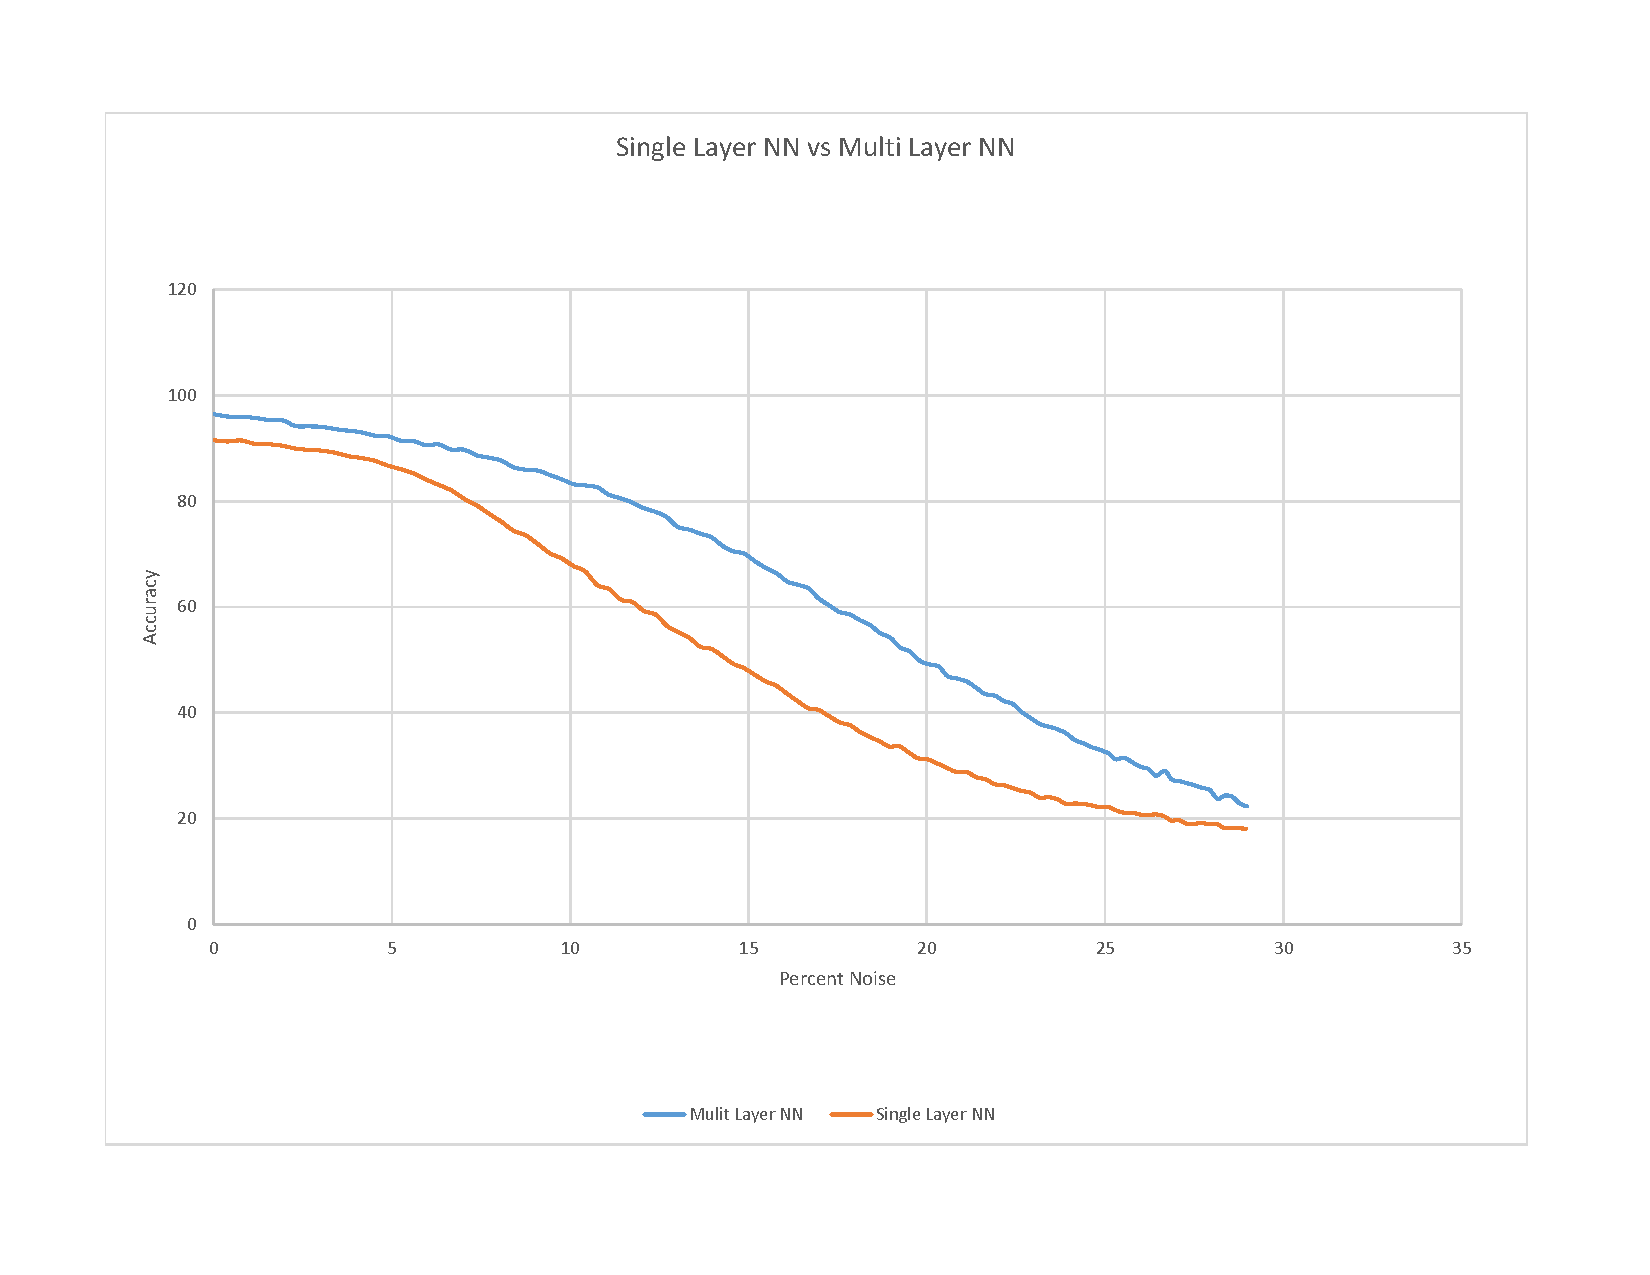
\includegraphics[width=\linewidth]{SinglevsMulti.pdf}
				\caption{A plot of accuracy loss over percent noise for both neural nets where the orange and blue lines represent the single and multi-layer neural nets respectively.}
				\label{part1}
			\end{figure}
			
		\subsection{Part 2}
			For part two only pictures of 0's and 1's were used due to a limitation of the hopfield network. For this data subset, a control accuracy was established at around 97\% and 98\% for both the single layer and multi-layer neural nets respectively for clean data and 95\% accuracy for hopfield data for both types of neural nets. Once the control was established, averages of the images needed to be calculated. Image ``averages" were calculated by pixel-wise adding all of the pictures of the same type and dividing the results by the number of pictures used. These averages are used to train the hopfield network's weight matrix. Next an image had the noise function applied to it. This image was run through both the neural net and accuracy was determined and then hopfield net and neural net to compare side by side results of the performance of the two mechanisms.
			
			The results for this experiment were quite remarkable. For both types of neural nets, the accuracy decay without using the hopfield network resembled that of part 1, quick accuracy loss. However, when the data was run through the hopfield network first, the accuracy of the neural nets was maintained far longer than through the non-hopfield test. Accuracy was held around 95\% through about 20\% noise in the data sets.
			
			\begin{figure}
				\centering
				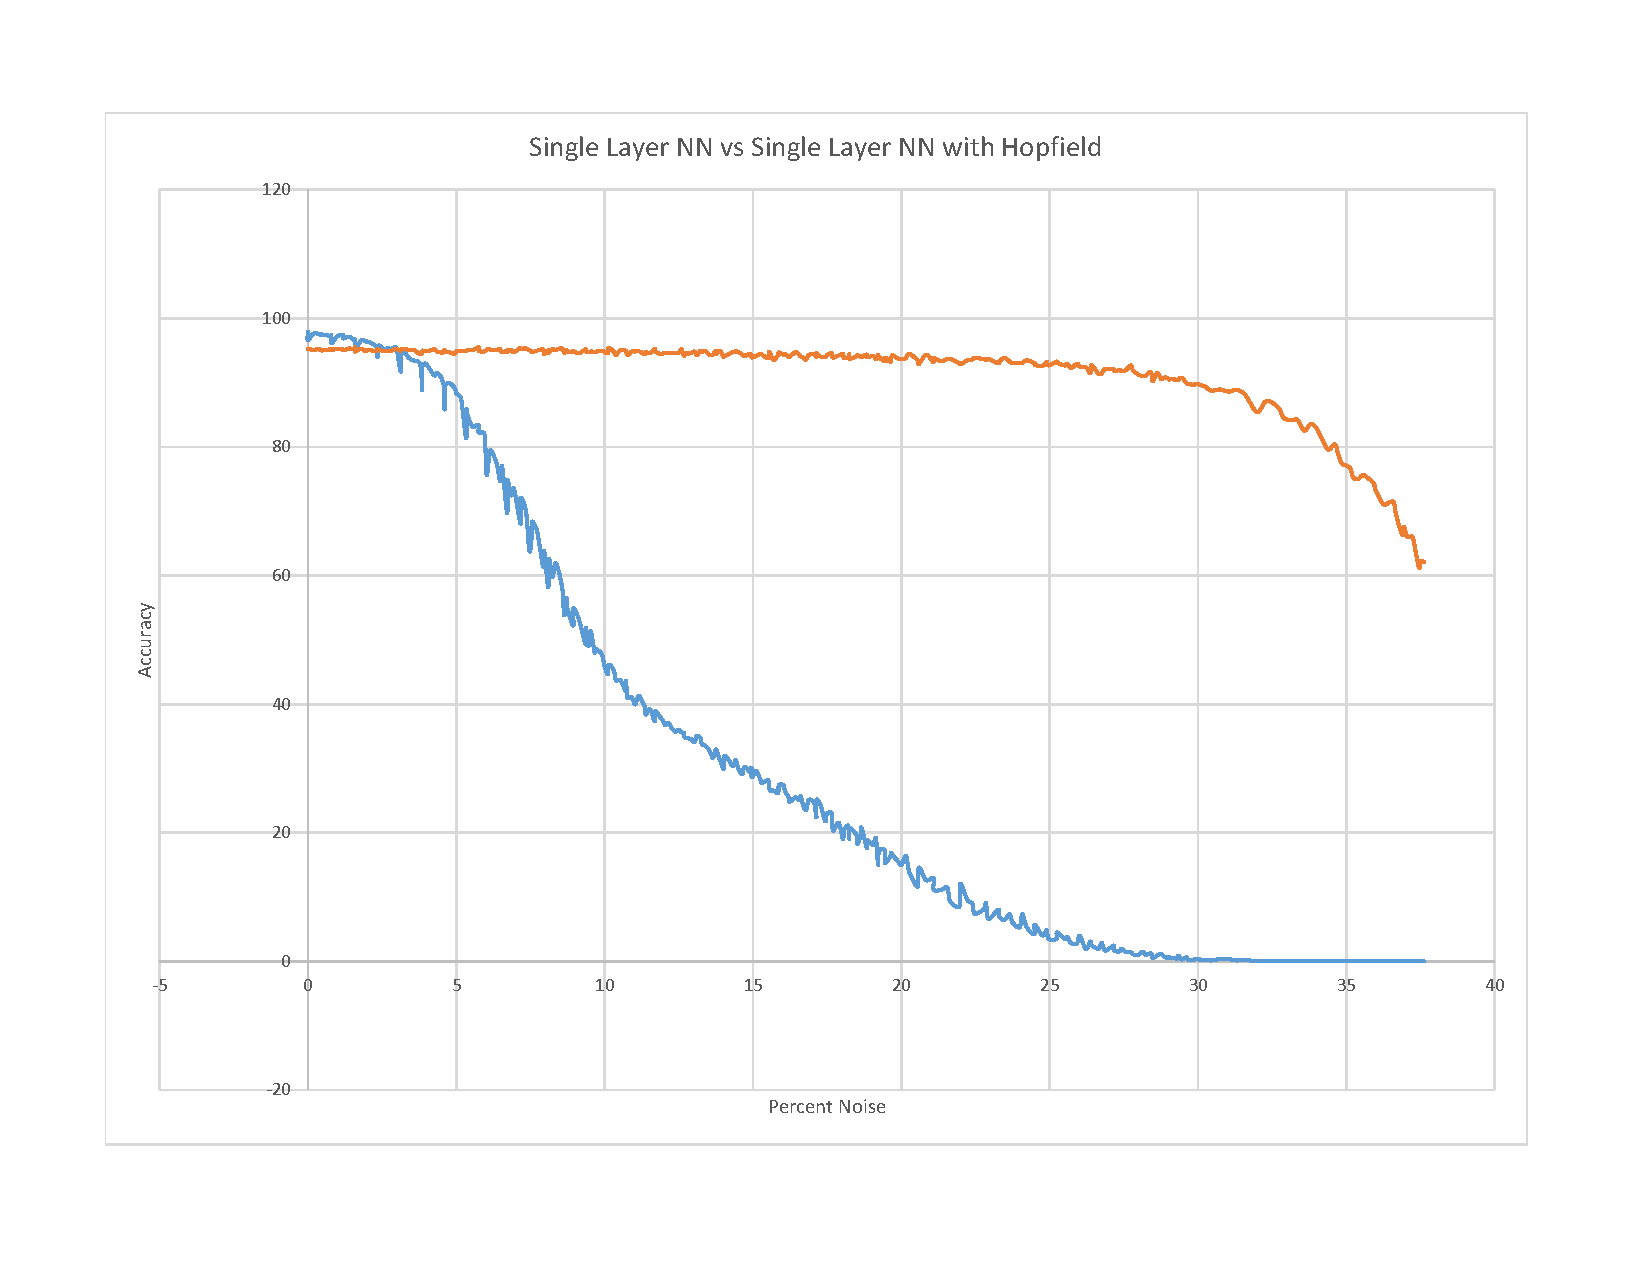
\includegraphics[width=\linewidth]{SingleLayerHop.pdf}
				\caption{A plot of accuracy over noise for the single layer hopfield test. The blue line is the control line and the orange line is the accuracy when the data is run through the hopfield network.}
				\label{part2A}
			\end{figure}
			
			\begin{figure}
				\centering
				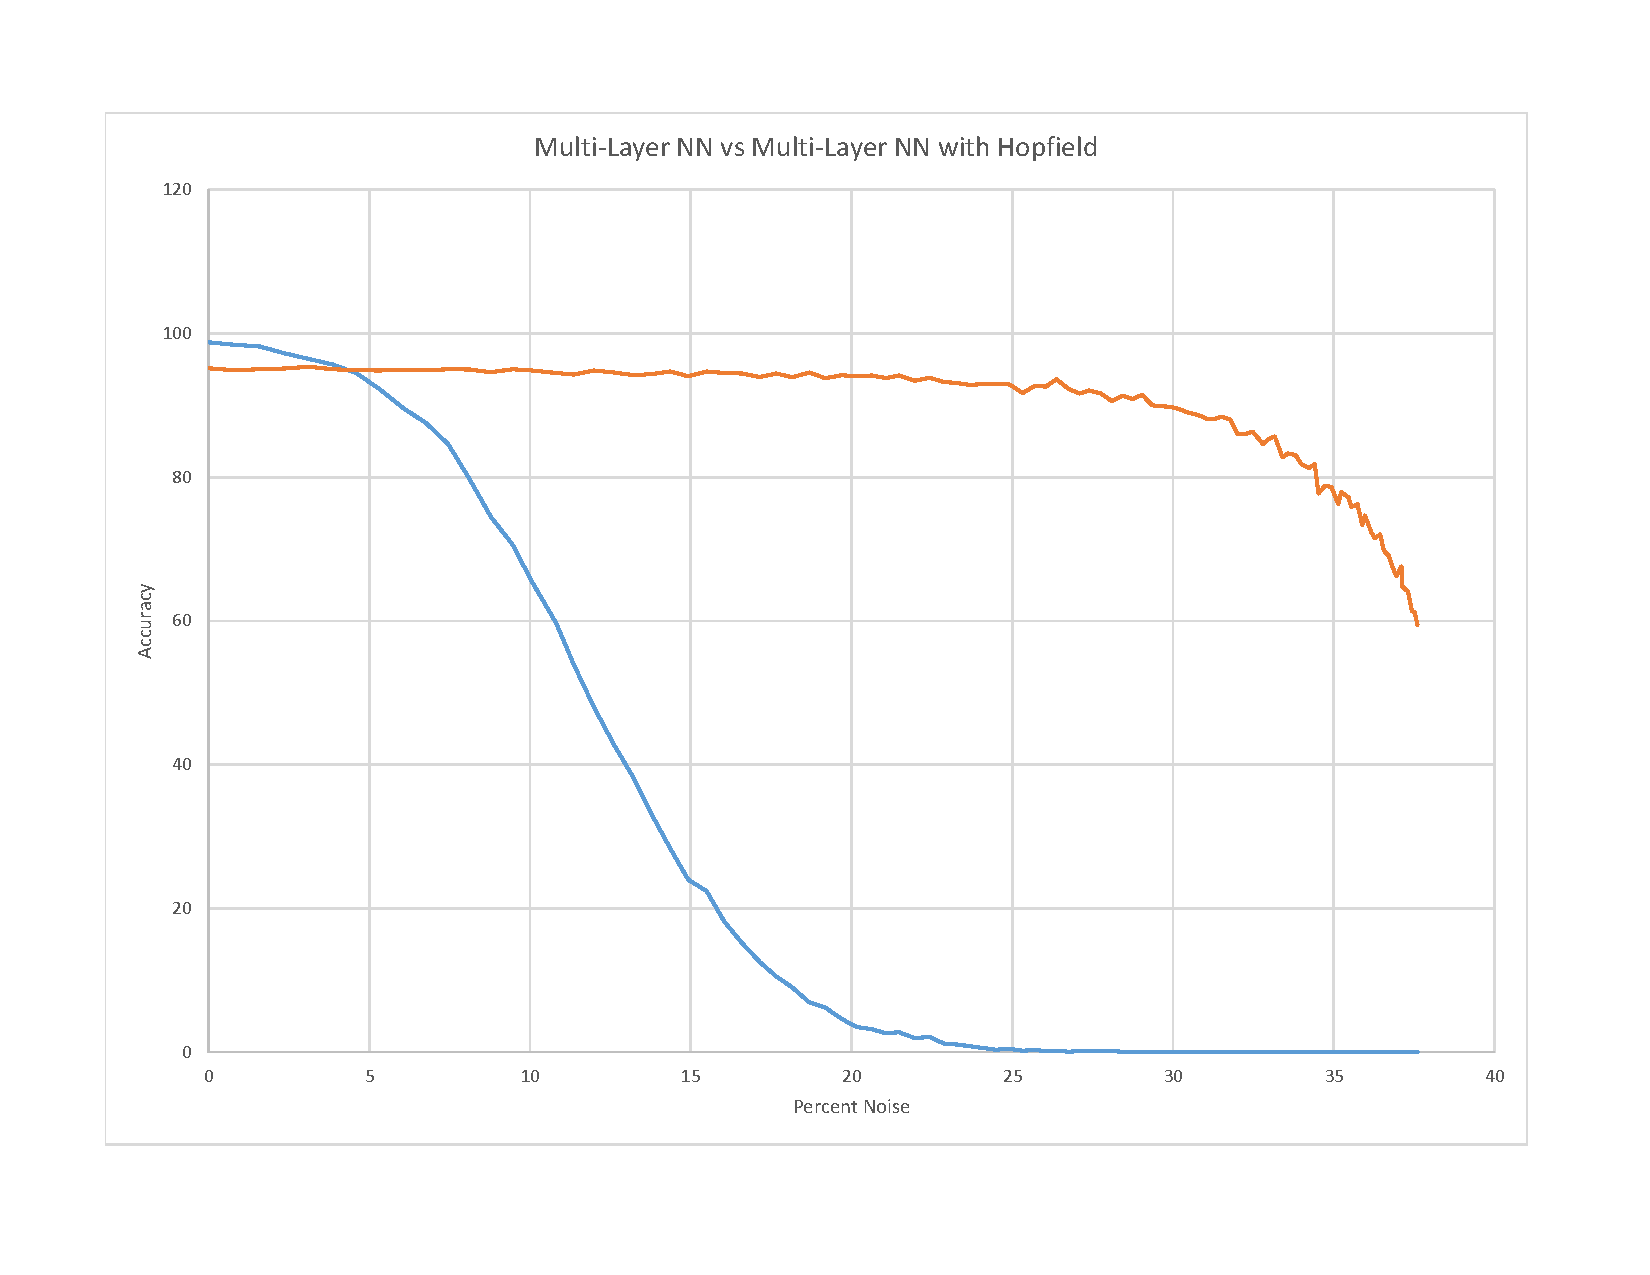
\includegraphics[width=\linewidth]{MultiLayerHop.pdf}
				\caption{A plot of accuracy over noise for the multi-layer hopfield test. The blue line is the control line and the orange line is the accuracy when the data is run through the hopfield network.}
				\label{part2B}
			\end{figure}
			
			Figures \ref{part2A} and \ref{part2B} show plots of the results of the two experiments. It can be seen the that accuracy of running the data through the hopfield network hold even after total accuracy loss of the neural nets. Its not until after 30\% noise injection into the data points that the hopfield begins to really lose its accuracy. 			
			
	\section{Conclusion}
		The results of this experiment might suggest that preset data may be better understood when first run through a hopfield network if the data is expected to be subject to interference. New techniques in clearing up communication noise in remote control settings can be established due to the well-defined functionality of the controls. Taking drones for example, the number of commands that are sent to a drone are generally well defined and can be trained into a hopfield network. If an established set of commands are defined for a drone then a system such as this one can be used to clear up noisy communication channels allowing for better control. 
		
		I believe that the overall question of ``can a hopfield neural network combination filter out noise better than a neural network alone" has successfully been answered with this experiment. I learned that hopfield networks can be tricky when training with exceedingly similar data points but also that they can be a powerful counterpart to various machine learning applications.
	
	\bibliographystyle{IEEEtran}
	\bibliography{ref}
\end{document}